\section{Durchführung}
\label{sec:Durchführung}

\subsection{Bestimmung einer Durchlasskurve}
Die Durchlasskurven einer LC- beziehungsweise LC$_1$C$_2$-Kette können
mit dem Aufbau in Abbildung \ref{fig:durchlasskurve} bestimmt werden.
\begin{figure}
    \centering
    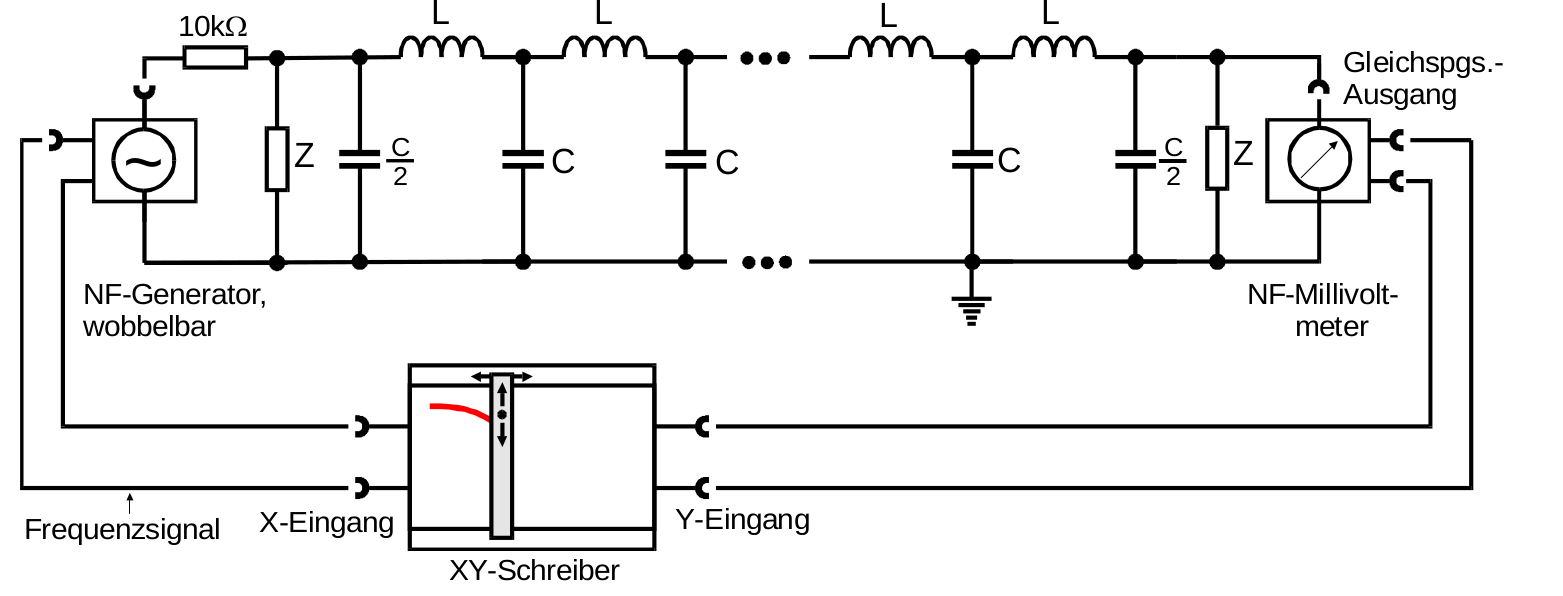
\includegraphics[width=0.8\textwidth]{Bilder/durchlasskurve.png}
    \caption{Versuchsaufbau zur Bestimmung der Durchlasskurven der $LC$-bzw. $LC_1C_2$-Kette. \cite{Anleitung}}
    \label{fig:durchlasskurve}
\end{figure}
Der Wellenwiderstand $Z$ am Eingang und Ausgang der Kette wird durch einen
regelbaren Widerstand realisiert und mittels
\begin{equation}
	Z = \sqrt{\frac{L}{C}}
\end{equation}
beziehungsweise
\begin{equation}
	Z = \sqrt{\frac{2L}{C_1+C_2}}
\end{equation}
auf den genäherten Wellenwiderstand $Z$ für kleine Frequenzen festgelegt (vergleiche Formel \eqref{eqn:wellenwiderstand}).
Auf einem X-Y-Schreiber lässt sich die Ausgangsspannung $U_{\text{aus}}$ in Abhängigkeit von der Frequenz $\omega$ der Eingangsspannung $U_{\text{ein}}$ aufzeichnen.
Die Eingangsspannung liefert ein wobbelbarer NF-Generator.
Außerdem kann an diesem NF-Generator eine Range eingestellt werden, in der die Frequenzen um eine festgelegte Frequenz variieren.
Dies ermöglicht eine Aufzeichnung um die Grenzfrequenz -- beziehungsweise
bei der LC$_1$C$_2$-Kette um die Grenzfrequenzen.

Des Weiteren müssen an dem X-Y-Schreiber die Position sowie die Sensitivität der Achsen eingestellt werden.
Hierbei muss beachtet werden, dass der Schreiber nicht den Rand überschreitet und der betrachtete Messbereich geeignet groß dargestellt wird.

Nachdem die Kalibrierung abgeschlossen und die Grenzfrequenzen zu erkennen sind, kann der Aufzeichnungsvorgang am X-Y-Schreiber gestartet werden.
Bei diesem müssen einige Referenzpunkte für die Frequenz bestimmt werden,
da die Achsen des verwendeten Millimeterpapiers nicht skaliert sind.

Bei der Aufzeichnung der Durchlasskurve für die LC$_1$C$_2$-Kette wird jeder zweite Kondensator der LC-Kette durch einen Kondensator mit anderer Kapazität ersetzt.


\subsection{Dispersionsrelation}
\label{sec:dispi}

Hierbei soll die Frequenzabhängigkeit der Phasenverschiebung $\phi$
zwischen Eingangsspannung $U_{\text{ein}}$ und Ausgangsspannung $U_{\text{aus}}$ gemäß der Dispersionsrelation nach Formel \eqref{eqn:dispersion}
-- beziehungsweise Formel \eqref{eqn:dispersion2} untersucht werden.
Zum Nachweis der Dispersionsrelation lässt sich der Aufbau aus Abbildung
\ref{fig:dispersionsrealtion} verwenden.
\begin{figure}
    \centering
    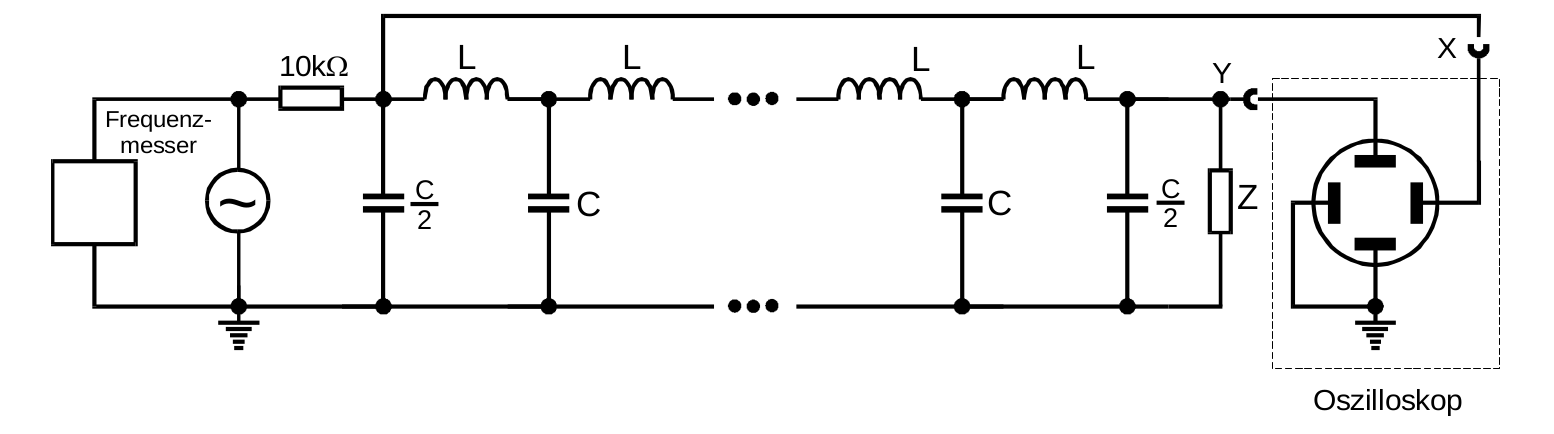
\includegraphics[width=0.8\textwidth]{Bilder/dispersionsrelation.png}
    \caption{Versuchsaufbau zur Bestimmung der Dispersionsrelation. \cite{Anleitung}}
    \label{fig:dispersionsrealtion}
\end{figure}
Dafür wird die Eingangsspannung sowie die Ausgangsspannung auf den X- beziehungsweise Y-Eingang
des Oszilloskops gegeben und das Oszilloskop im Zwei-Kanal-Modus betrieben.
Dann werden für die LC- und die LC$_1$C$_2$-Kette die Frequenzen ermittelt, bei denen auf
dem Oszilloskop eine Phasenverschiebung von $\pi$ zu erkennen ist.
Dies wird realisiert, indem am NF-Generator die Frequenzen $\omega$ der Eingangsspannung
hochgeregelt werden bis auf dem Oszilloskop eine Phasenverschiebung von $\pi$ also eine
Gerade zu erkennen ist.


Zu beachten ist hier, dass bei der LC$_1$C$_2$-Kette -- wie in Abschnitt \ref{subsec-dispersion} erläutert

-- der optische Ast auftritt.


\subsection{Nachweis von stehenden Wellen}

Stehende Wellen können mit der Schaltung aus Abbildung \ref{fig:durchlasskurve} nachgewiesen
werden, wobei der X-Y-Schreiber, die Wobbeleinrichtung sowie die Wellenwiderstände $Z$ entfernt
werden. Die entfernten Wellenwiderstände sorgen für offene Enden der stehenden Welle am Anfang
und am Ende der Kette, wodurch ein Spannungsmaximum am Anfang und am Ende der Kette zu erkennen
sein sollte, wenn die Eigenfrequenzen der beiderseits offenen LC-Kette angelegt sind.

Diese Eigenfrequenzen sollen auch bestimmt werden, indem -- wie bei der Bestimmung der Phasenverschiebung in Abschnitt \ref{sec:dispi} --
die Frequenz $\omega$ der Eingangsspannung hochgeregelt wird, bis Maxima am Anfang und am Ende der LC-Kette auftreten. Die ermittelten Eigenfrequenzen werden abgelesen und notiert.

Weiterhin sollen die einzelnen Kettenglieder bei den ersten beiden Eigenfrequenzen näher betrachtet werden, indem jeweils die Spannungsamplitude mit einem Millivoltmeter bestimmt wird.
Das Millivoltmeter kann mit Hilfe eines Stufenschalters nacheinander an die einzelnen
Kettenglieder geschaltet werden und so die Spannungsamplituden messen.

Zuletzt sollen die Spannungsamplituden der einzelnen Kettenglieder (bei einer Frequenz) bei angebrachtem Wellenwiderstand -- also bei einer LC-Kette mit geschlossenen Enden -- analog wie bei der Messung zuvor bestimmt werden.
